\documentclass{tufte-handout}
\usepackage[utf8]{inputenc}
\usepackage{amssymb, fdsymbol, mathtools, amsthm, amsmath} % Varios paquetes de símbolos
\usepackage{titling} % Para estilizar el título
\usepackage{lastpage}
\usepackage{fancyhdr} % Para hacer encabezados y pie de página más estilizados
\usepackage{graphicx} % Maneja las imágenes
\usepackage{wrapfig, subcaption} % Para centrar las figuras y colocar subcaptions
\usepackage{float}
\usepackage{color} % Para usar colores en el texto
\usepackage{soul} % Para subrayar con colores
\usepackage{cancel} % Para tachar expresiones

% Redefinimos los ambientes de teoremas, definiciones, etc.
\theoremstyle{plain}
\newtheorem{teo}{Teorema}
\newtheorem{cor}[teo]{Corolario}
\newtheorem{lem}[teo]{Lema}
\newtheorem{pro}[teo]{Proposición}
\newtheorem{pre}{Pregunta}

\theoremstyle{definition}
\newtheorem{defn}{Definición}
\newtheorem{ejem}{Ejemplo}
\newtheorem{ejer}{Ejercicio}
\newtheorem{notn}{Notación}
\newtheorem{nota}{Nota}
\newtheorem{prob}{Problema}
\newtheorem{aco}{Acotación}

% Comandos para símbolos
\newcommand{\R}{\mathbb{R}}
\newcommand{\Z}{\mathbb{Z}}
\newcommand{\N}{\mathbb{N}}
\newcommand{\C}{\mathbb{C}}
\newcommand{\Parts}{\mathcal{P}}

% Cambia el nombre de varios comandos
\renewcommand{\contentsname}{Contenido}
\renewcommand*{\proofname}{Demostración}
\renewcommand{\figurename}{Fig.}
\renewcommand{\refname}{Referencias}

% Resetea el contador de ecuaciones en cada sección
\newcounter{sec}
\setcounter{sec}{0}
\counterwithin*{equation}{sec}
\counterwithin*{ejer}{sec}

% Establece el subrayado de color rojo
\definecolor{ferrari}{rgb}{1,0.17,0}
\setulcolor{ferrari}

% Reduce el espacio entre el título y el header
\setlength{\droptitle}{-5.5em}
\renewcommand\maketitlehookc{\vspace{-3ex}}

% Define el espaciado entre párrafos
\setlength{\parskip}{1.5em}

% Establecemos cómo será el encabezado y el pie de página
\fancyhf{}
\pagestyle{fancy}
\fancyhf{}
\fancyhead[L]{MA-3323}
\fancyhead[C]{Eduardo José Gavazut Pinto}
\fancyhead[R]{13-10524}
\fancyfoot[L]{Sección 1}
\fancyfoot[R]{Profesor: Iris López}
\fancyfoot[C]{\thepage\ de \pageref{LastPage}}
\renewcommand{\headrulewidth}{2pt} 
\renewcommand{\footrulewidth}{2pt}

% Definir el título
\pretitle{\begin{flushleft}\LARGE\sffamily}
\title{
Notas de Análisis VI, Universidad Simón Bolívar
}
\posttitle{\par\end{flushleft}\vskip 0.5em}
\preauthor{\begin{flushleft}\large\scshape}
\author{Eduardo Gavazut, Carnet: 13-10524}
\postauthor{\par\end{flushleft}}
\predate{\begin{flushleft}\large\scshape}
\date{Enero-Marzo 2024}
\postdate{\par\end{flushleft}}

% Aquí empieza el documento
\begin{document}

\maketitle
\thispagestyle{fancy}
\tableofcontents

\newpage
\subsection{Eficiencia de un algoritmo}

Con lo anterior, tenemos claro que una tarea se puede llevar a cabo mediante distintos algoritmos, entonces ¿cuál es el mejor?. Podemos asignarle una \textbf{medida} o un \textbf{tamaño} a un \textbf{caso} (o instancia). Y esto es subjetivo. Por ejemplo, para calcular la suma de dos números naturales $a$ y $b$ podemos asignar como medida del caso la cantidad de dígitos del máximo entre $a$ y $b$. Luego analizamos cuántas operaciones significativas se deben hacer en función de esa medida. Usando el algoritmo de adición básico:

\begin{center}
    \begin{tabular}{ccccccccccc|c}
            &   & 7 &   & 8 &   & 1 &   & 5 &   & 3 & $a$            \\
        $+$ &   & 3 &   & 7 &   & 4 &   & 2 &   & 9 & $b$            \\ \midrule
            & 1 &   & 1 &   & 0 &   & 0 &   & 1 &   & \text{llevo}   \\
         1  &   & 1 &   & 5 &   & 5 &   & 8 &   & 2 & $s$    
    \end{tabular}
\end{center}

\noindent entonces en el \textbf{peor de los casos}, si ambos números tienen $n$ dígitos, tendremos que ejecutar $n$ adiciones de números pequeños (es decir de un dígito) y una que otra adición más (cuando \textit{llevamos}). Nos guiamos por el peor de los casos.\marginnote{De igual manera, el algoritmo (usual) de la multiplicación de dos números naturales, si volvemos a tomar como medida de la instancia la cantidad de dígitos del mayor número, el algoritmo tiene eficiencia $n^2$. Ya que consideramos que las operaciones significativas son las multiplicaciones de un dígito.}


\begin{ejem}
    El siguiente algoritmo arroja la representación binaria del número $m$ dado en su     forma decimal.
    
    \begin{algoritmo}
    \caption{Representación binaria de un número en forma decimal}\label{alg:bin}
    \KwData{$y > 0$}
    \KwResult{$N_2$, representación binaria de $m$}
    $y \leftarrow N$\;
    $i \leftarrow 0$\;
    \If{$y = 0$}{
    \Return{$N_2 \leftarrow 0$}
    }
    \While{$y \neq 0$}{
        \eIf{$y$ \textup{es par}}{
            $r_i \leftarrow 0$\;}{
            $r_i \leftarrow 1$\;
            $y \leftarrow y-1$\;}
        $y \leftarrow y/2$\;
        $i \leftarrow i+1$\; 
    }
    $t \leftarrow i-1$\;
    \Return{$N_2 \leftarrow r_tr_{t-1}r_{t-2} \dots r_1r_0$}
    \end{algoritmo}
    
    \noindent el proceso es como se muestra a continuación, y termina cuando el cociente es cero
    
    \begin{gather*}
        N = 2 \cdot q_0 + r_0 \\
        q_0 = 2 \cdot q_1 + r_1 \\
        \vdots \\
        q_{t-2} = 2 \cdot q_{t-1} + r_{t-1} \\
        q_{t-1} = r_t \quad (q_i = 0)
    \end{gather*}
    
    \noindent luego la representación binaria es $r_tr_{t-1} \dots r_1r_0$. Si el tamaño de la instancia es la cantidad de dígitos de $m$\marginfootnote{En el Biggs, se consideran dos posibles medidas para el tamaño: el valor de $m$ como tal, o su cantidad de dígitos}, digamos
    
    \[
    m = x_{n-1}x_{n-2}\dots x_1x_0 \quad \text{en base 10}
    \]
    
    \noindent entonces $10^{n-1} < m \leq 10^n-1$, por lo que $n-1$ es la parte entera de $\log_{10}m$, por lo que el número $n$ de decimales en $m$ está dado por\marginnote{En el vídeo Nieto solo dice "aplicando logaritmo" en este paso. Esta explicación fue sacada directamente del libro (página 145).}
    
    \[
    n = \lfloor \log_{10}m + 1 \rfloor
    \]
    
    \noindent ahora, la operación más significativa es la división entre 2. ¿Cuántas veces?: pues $t+1$, que coincide con la cantidad de dígitos de la representación binaria. O sea, que tenemos
    
    \[
    t + 1 = \lfloor \log_2m \rfloor + 1 = \lfloor \log m / \log 2 \rfloor + 1 \quad \footnotemark
    \]\footnotetext{Se aplican propiedades de los logaritmos en este paso.}
    
    Así que $t+1$ en función de $n$ es aproximadamente $\frac{10}{3}n$. Sólo nos interesa el comportamiento de la eficiencia para valores grandes de $n$, por eso nos conformamos con una aproximación.
\end{ejem}

\subsection{Notación "$O$ grande"}

\begin{defn}    
    Dadas las funciones $f, g: \N \rightarrow \N$, decimos que $f$ es \ul{$O(g(n))$} si eventualmente
    
    \[
    f(n) \leq \lambda g(n)
    \]
    
    \noindent para algún $\lambda > 0$. Es decir, la desigualdad se cumple excepto para una cantidad finita de valores de $n$.
\end{defn}

\begin{ejem}
    Consideremos lo siguiente
    
    \[
    3n^3 + 20n^2 + 5n + 11 \leq (3 + 20 + 5 + 11)n^3 = 39n^3
    \]
    
    \noindent así que $f(n) = 3n^3 + 20n^2 + 5n + 11$ es $O(n^3)$. También $2^n + 3n^5 + 12n^4$ es $O(2^n)$.
\end{ejem}

\begin{nota} 
    Hay que tener presente lo siguiente:
    
    \begin{enumerate}
        \item Decir que $f(n)$ es $O(g(n))$ \textbf{no significa} que $f(n) = O(g(n))$ (esto ni sentido tiene).
        \item Si $f(n)$ es $O(g(n))$ y $h$ es una función que supera a $g$, entonces $f(n)$ también es $O(h(n))$. Por ejemplo, si $f(n)$ es $O(n^4)$, entonces también es $O(n^7)$. Pero la idea es buscar una opción óptima para $g$ cuando analizamos la eficiencia de algoritmos.
    \end{enumerate}
\end{nota}

\subsection{Comparar algoritmos}

Veamos, como ejemplo que se puede mejorar (respecto a la eficiencia) el algoritmo usual para calcular la $m$-ésima potencia de un número natural dado: Para calcular $x^m$, multiplicamos $x$ por $x$ sucesivamente, con un total de $m-1$ multiplicaciones. Si la medida de la instancia es la cantidad de $n$ dígitos de $m$, ya vimos que

\[
n = \lfloor \log m \rfloor
\]

\noindent así que $m$ es aproximadamente $10^n$. Por lo tanto este algoritmo tiene eficiencia $O(10^n)$.

Un caso particular nos muestra un atajo para calcular la potencia de manera más eficiente. Por ejemplo $x^{23}$ se puede calcular así:

\begin{enumerate}
    \item Calcula $x^2$, $x^4$, $x^8$, $x^{16}$ (cuatro multiplicaciones).
    \item Calcula $x \cdot x^2$, $x^3 \cdot x^4$, $x^7 \cdot x^{16}$ (tres multiplicaciones).
\end{enumerate}

Esto es mejor que las 22 multiplicaciones que requiere el primer algoritmo. Ahora, se observa que $x^{23} = x^{16+4+2+1}$, y tenemos que 23 está representado como una suma de potencias de 2, lo cual lleva a la representación binaria de 23, o sea 10111. El diagrama nos ayuda ver el proceso sugerido:

\begin{center}
    \begin{tabular}{ccccccccccc|c}
               &            & $x^{16}$   &              & $x^8$ &            & $x^4$      &            & $x^2$      &            & $x$        & \text{techo}  \\
               & $\swarrow$ & $\uparrow$ &              &       & $\swarrow$ & $\uparrow$ & $\swarrow$ & $\uparrow$ & $\swarrow$ & $\uparrow$ &               \\
        $x^{23}$ &            & $x^{7}$    & $\leftarrow$ & $x^7$ &            & $x^3$      &            & $x$        &            & 1          & \text{piso}   \\
               &            & 1          &              & 0     &            & 1          &            & 1          &            & 1          & \text{sótano}
    \end{tabular}
\end{center}

Lo leemos de derecha a izquierda: Comenzando con el 1 en la fila \textbf{piso}, si el número en el sótano es 1, multiplicamos por el valor en el \textbf{techo}. Este será el nuevo valor en el \textbf{piso}. Si el número en \textbf{sótano} es 0, el valor en piso se mantiene. El algoritmo sería:

\begin{algoritmo}
    \caption{Potencia}\label{alg:pot}
    \KwData{$x$ base de la potencia, $n$ potencia}
    \KwResult{$x^n$}
    
    piso $= 1$\:
    techo $= x$\;
    \While{$n > 0$}{
    \If{$n\%2 == 1$}{
    piso $=$ piso $*$ techo\;
    }
    techo $=$ techo $*$ techo\;
    $n = n // 2$\;
    }
    \Return{\textup{piso}}
\end{algoritmo}

\begin{pre} ¿Cuál es la eficiencia de este algoritmo?: \end{pre}

\begin{enumerate}
    \item La cantidad de dígitos en la representación binaria de $m$ es aproximadamente $\log_2 m$.
    \item El algoritmo hace a lo sumo $2(\log_2 m-1)$ multiplicaciones.
    \item Como $n = \lfloor \log m \rfloor$, la relación es lineal. O sea, la eficiencia es $O(n)$\marginfootnote{En el libro dice que la eficiencia es $O(\log n)$, revisar con Nieto.}.
\end{enumerate}

Para este algoritmo, no podemos obtener una mejora significativa para calcular $x^n$. Esto se debe a que cada multiplicación a lo más puede doblar el exponente más grande obtenido hasta ese momento, por lo que $r$ multiplicaciones no nos pueden llevar más allá de $m^{2r}$. En consecuencia, cuando $n = 2^r+1$, el número de multiplicaciones que se requieren para cobtener $m^n$ es al menos $r+1$, lo que es aproximadamente $\log_2 n$. Por lo que la eficiencia de cualquier algoritmo para este problema es al menos $O(\log n)$.

\subsection{Algoritmos de ordenamiento}

Tenemos a la mano el siguiente problema: Dado un conjunto de datos $x_1, \dots, x_n$, queremos ordenarlo de manera creciente (o decreciente). Es decir, queremos hallar una \textbf{permutación} $\sigma$ de $\{1, 2, \dots, n\}$ tal que

\[
x_{\sigma_{(1)}} < x_{\sigma_{(2)}} < \dots < x_{\sigma_{(n)}}
\]

Para resolver este problema, analizaremos dos algortimos básicos:

El \textbf{algoritmo de la burbuja} compara el primer elemento del conjunto con el segundo, si no están en el orden adecuado entonces los intercambia. Luego hace lo mismo con el segundo y el tercero. Y así sucesivamente hasta hacerlo con los dos últimos elementos. Al terminar esta etapa, queda el mayor de los elementos en la última posición. Luego se procede de la misma manera con los primeros elementos del conjunto (sin el último). Así hasta que haya que comparar únicamente a los dos primeros elementos.

\begin{figure}[h]
    \centering
    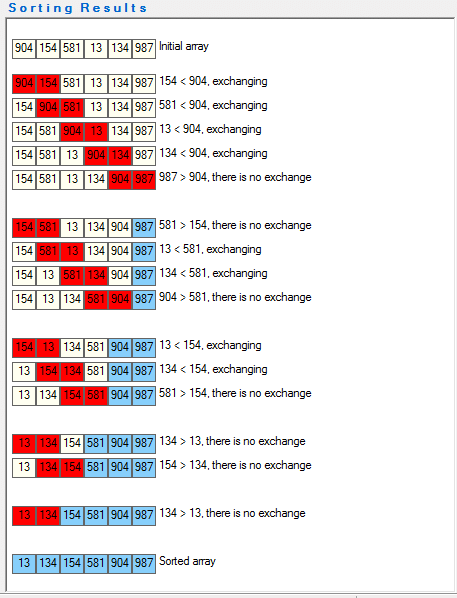
\includegraphics[scale=0.5]{img/Obtained-result-using-Bubble-sort-algorithm-and-array-with-six-elements.png}
    \caption{Corrida de Bubble Sort para un arreglo no ordenado (imagen sacada de Google).}
\end{figure}

A continuación, el código para el algoritmo de la burbuja\marginfootnote{Pseudocódigo sacado del Cormen.}:

\begin{algoritmo}
    \caption{Bubble Sort}\label{alg:bubble}
    \KwData{$A$ arreglo no ordenado}
    \KwResult{$A$ arreglo ordenado}
    \For{$i \leftarrow 1$ \textup{hasta} $length[A]$}{
        \For{$j \leftarrow length[A]$ \textup{hasta} $i+1$}{
        \If{$A[j] < A[j-1]$}{
        intercambia $A[j] \rightleftarrows A[j-1]$
        }
        }
    }
\end{algoritmo}

\break

Analicemos el algoritmo. Las operaciones son comparaciones e intercambio de valores. Así que, si el conjunto tiene $n$ elementos y esa es la medida de la instancia:

\begin{itemize}
    \item Para cada $j$ se hacen $n - j - 1$ comparaciones.
    \item Son $(n-1) + (n-2) + \dots + 2 + 1 = \frac{1}{2}n(n-1)$.
    \item Esto es $O(n^2)$.
    \item La cantidad de intercambios es también $O(n^2)$ (esto en el peor de los casos, se hace un intercambio después de cada comparación).
\end{itemize}

\textbf{En conclusión:} El algoritmo de la burbuja tiene eficiencia $O(n^2)$ en función de la cantidad de elementos del conjunto a ordenar.

Comparemos el algoritmo de la burbuja con una versión del algoritmo de inserción. El \textbf{algoritmo de inserción} construye una lista comenzando con el primer elemento del conjunto dado. Luego agrega el segundo elemento a la lista \textit{en el lugar correcto}. Y así sigue con los demás elementos del conjunto de manera que cada lista queda ordenada de una vez. La eficiencia de este algoritmo depende del método que se utilice para insertar el elemento \textit{en el lugar correcto}.

En nuestro caso, usaremos el método de \textbf{bisección}: Para insertar el $i$-ésimo elemento, se decide en cuál mitad de la lista debería ir. Después, en cuál mitad de esa mitad debería ir y así sucesivamente.

Ahora, analicemos este algoritmo:

\begin{itemize}
    \item Supongamos que el conjunto a ordenar tiene $n$ elementos.
    \item Si $n$ está entre $2^{r-1}$ y $2^r$, entonces hay que hacer $r$ comparaciones.
    \item En total son $\log_22 + \log_23 + \dots + \log_2 n$ comparaciones (aprox.).
    \item Esto es $O(n\log n)$.
\end{itemize}

\textbf{En conclusión}: El algoritmo de inserción, usando el método de bisección tiene eficiencia $O(n \log n)$. Pero al hacer la inserción en el lugar correcto, en el peor de los casos hay que intercambiar los términos de la lista. Esto serían otra vez $n^2$ intercambios. Por tanto, este algoritmo tiene también eficiencia $O(n^2)$.
Lo que hemos hecho es probar un caso particular de un resultado que se le debe a F.P Ramsey. Enunciemos el teorema de Ramsey de la siguiente manera:

\begin{teo}[Ramsey (TR)]\label{teo:TR}
    Para todo $n \in \N$ y todo $k \in \N$
    
    \[
    \omega \rightarrow (\omega)_r^n
    \]
\end{teo}

\begin{proof}
    Procedamos igual que en la demostración anterior con un argumento inductivo: El caso $r=1$ es trivial, así que pasemos a demostrar el caso $r=2$ con inducción sobre $n$.
        
    Si $n=1$, nuevamente es trivial; si $n=2$, ya hemos hecho la demostración en \ref{pre:ramsay1}. Supongamos entonces que el teorema vale para $n$ y probemos para $\omega \rightarrow (\omega)_2^{n+1}$. Como $\N$ es un conjunto infinito numerable, estudiar sus coloraciones vale para cualquier conjunto infinito numerable, así que por conveniencia nos quedaremos estudiando $\N$. Luego, tendremos $f: \N \rightarrow 2$, y nuestro objetivo será conseguir un conjunto homogéneo para $f$.
    
    \begin{marginfigure}
        \centering
        \begin{forest}
            [$0$, for tree={grow=90}, red
                [$1$, red
                    [\vdots
                        [$n-1$, red
                            [$X_1$
                                [$Y_3$
                                    [\vdots]
                                ]
                                [$Y_2$
                                    [\vdots]
                                ]
                            ]
                            [$X_0$
                                [$Y_1$
                                    [\vdots]
                                ]
                                [$Y_0$
                                    [\vdots]
                                ]
                            ]
                        ]
                    ]
                ]
            ]
        \end{forest}
        \caption{Representación de la construcción del árbol construído en la demostración del teorema de Ramsey.}
        \label{fig:ramseyfig1}
    \end{marginfigure}
    
    Entonces, construyamos un árbol de la siguiente manera: Sabemos que los primero $n$ elementos tienen el mismo color, es decir $f(n-1) = i$, donde $i = 0$ o $i = 1$. Definamos entonces dos particiones de $\N$, $X_0$ y $X_1$ tales que
    
    \[
    t \in X_i \iff f\left( n \cup \{t\} \right) = i, \quad i \in \{0,1\}
    \]
      
    \noindent ahora, partiremos ambos conjuntos $X_0$ y $X_1$ de la siguiente manera: Sea $t_0 \in X_0$ el menor elemento de $X_0$ y consideremos $C_{t_0} = \pred(t_0) \cup \{t_0\}$, definiremos dos conjuntos $Y_0$ y $Y_1$ tales que
    
    \[
    t \in Y_i \iff f\left( x \cup \{t\} \right) = i, \quad \forall x \in C_{t_0}^{[n]}
    \]
    
    Supongamos que en este árbol que hemos estado construyendo, tenemos en el nivel $m$ a un elemento $s$, ¿cómo es la partición del conjunto al que pertenece?. Pues consideremos $C_{s} = \pred(t_0) \cup \{s\}$ y sean entonces $Z_0$, $Z_1$ dichas particiones definidas de esta manera:
    
    \[
    t \in Z_i \iff f\left( x \cup \{t\} \right) = i, \quad \forall x \in C_{s}^{[n]}
    \]
    
    Los sucesores inmediatos de $s$ son elegidos de tal forma que tomamos el menor de cada $Z_i$. Entonces cada elemento del nivel $m$ tiene a lo sumo $2^{\binom{m}{n}}$ sucesores inmediatos, ya que para cada elemento del nivel $m$, $\left| C_s^{[n]} \right| = \binom{m}{n}$ y tenemos 2 colores.
    
    Para cada uno de los pares de particiones que hemos construído, puede ocurrir que uno de ellos sea vacío, pero no que los dos sea vacío. Esto es así por la cardinalidad de $\N$.
    
    Como resultado, hemos construído inductivamente un árbol $T$ infinito donde cada nivel es finito, entonces por el teorema \ref{teo:arboles1}, existe una rama $R \subset T$ infinita. Ahora, sea $x \in R^{[n]}$, para todo $s > n$, $t > s$, por construcción tenemos que
    
    \[
    f\left(x \cup \{s\}\right) = f\left(x \cup \{t\}\right)
    \]
    
    Con esto, podemos definir una nueva partición $g: R^{[n]} \rightarrow 2$, donde
    
    \begin{gather*}
        g(x) = 0, \quad \text{si} \quad f(x) = 0 \\
        g(x) = 1, \quad \text{si} \quad f(x) = 1
    \end{gather*}
    
    Luego, recordemos que por hipótesis inductiva, $\omega \rightarrow (\omega)_2^{n}$ y $g$ cumple las condiciones para la hipótesis inductiva. De esta manera, hay un $H \subset R$ infinito tal que $H^{[n]}$ es monocromático para $g$, y por lo tanto monocromático para $f$.
    
    De esta forma, hemos demostrado el caso $r=2$. Supongamos ahora que el teorema es válido para $r \leq k$, es decir que $\omega \rightarrow (\omega)_r^n$ es válido para todo $n$. Sea ahora $f: \N^{[n]} \rightarrow k+1$, podemos definir otra partición auxiliar $G: \N^{[n]} \rightarrow 2$ definida como
    
    \begin{gather*}
        G(x) = 0, \quad \text{si} \quad f(x) = 0 \\
        G(x) = 1, \quad \text{si} \quad f(x) = 1
    \end{gather*}
    
    \noindent entonces, por hipótesis inductiva, $G$ tiene un conjunto homogéneo $H$ infinito. Si $G\left( H^{[n]} \right) = 0$, $H$ es homogéneo para $f$. Si $G\left( H^{[n]} \right) = 1$, entonces $f|H^{[n]}$ es una partición de $k$ partes, y por hipótesis inductiva existe un conjunto $H' \subseteq H$ tal que es infinito y homogéneo. Este conjunto $H'$ también es homogéneo para $f$.
\end{proof}

Con esto demostrado, podemos pasar a demostrar una consecuencia de carácter finita del teorema de Ramsey:

\begin{teo}[Teorema de Ramsey finito (TFR)]\label{teo:TRF}
    Dados números enteros positivos $n, r$ y $m$, existe un entero positivo $N$ tal que
    
    \[
    N \rightarrow (m)_r^n
    \]
\end{teo}

\marginnote{La versión que se usará durante el transcurso del curso es la verión infinita del \TR}.

\begin{proof}
    Supongamos que el teorema no se cumple, es decir que para cada $N \in \N$, existe una coloración $f_N: N^{[n]} \rightarrow k$ tal que $\forall x \in N^{[m]}$, $x^{[n]}$ \textbf{no} es homogéneo para $f_N$.
    
    Con esto, definamos una función $f: \N^{[n+1]} \rightarrow k$ tal que para cualquier sucesión de números naturales $\{a_0, a_1, \dots, a_n\}$ tenemos
    
    \[
    f\left( \{a_0, a_1, \dots, a_n\} \right) = f_{a_n} \left( \{a_0, a_1, \dots, a_{n-1}\} \right)
    \]
    
    \noindent es decir, $f$ asigna a una sucesión creciente de $n+1$ elementos, la coloración será la que le asigne $f_{a_n}$ a los primeros $n$ elementos de esa lista.
    
    Luego, el \hyperref[teo:TR]{TR} nos dice que existe un $H \subset \N$ infinito tal que $H$ es homogéneo para $f$, con $H = \{h_0, h_1, \dots \}$. De esta forma, un conjunto $h$ de $m$ elementos tal que $h \subset H$ es también homogéneo para $f_{h_m}$. Al hacer la restricción $f_N|f_{h_m}$, tenemos que $h$ es homogéneo. Esto es una contradicción, ya que habíamos supuesto que no hay homogéneos de tamaño $m$ para $f_N$.
    
    Por lo tanto, el teorema de Ramsey finito es cierto.
\end{proof}
\begin{teo}[Teorema de la función implícita, generalización de la versión 3]
    Sea $F: \R^{n+m} \rightarrow \R^m$ diferenciable y de clase $C^2$, donde $F = (F_1, \dots, F_m)$ y a su vez $F_i(x_1, \dots, x_n, z_1, \dots, z_m)$. Consideremos $p_0 = (x_0, z_0) \in \R^{n+m}$. Consideremos también para cada $i = 1, \dots m$, $\Delta$ de la siguiente manera
    
    \[
    \Delta =
    \renewcommand\arraystretch{2}
    \begin{vmatrix}
        \frac{\partial F_1}{\partial z_1} & \dots & \frac{\partial F_1}{\partial z_m} \\
        \vdots & \ddots & \vdots \\
        \frac{\partial F_m}{\partial z_1} & \dots & \frac{\partial F_m}{\partial z_m}
    \end{vmatrix}
    \]
    
    \noindent donde cada derivada está evaluada en el punto $p_0$.
    
    Si tenemos que $F(p_0) = 0$ y $\Delta(p_0) \neq 0$, entonces en un entorno de $p_0$ tendremos que el sistema
    
    \[
    \begin{cases}
        F_1(x_1, \dots, x_n, z_1, \dots, z_m) = 0 \\
        \vdots \\
        F_m(x_1, \dots, x_n, z_1, \dots, z_m) = 0
    \end{cases}
    \]
    
    \noindent define de forma implícita a las funciones $z_i = f_i(x_1, \dots, x_n)$ con $i = 1, \dots, m$.
    
    Además, tendremos para $k = 1, \dots, n$ y $j = 1, \dots, m$
    
    \[
    \dfrac{\partial z_j}{\partial x_k} = -\dfrac{\dfrac{\partial(F_1, \dots, F_m)}{\partial(z_1, \dots, z_{j-1}, x_k, \dots, z_m)}}{\dfrac{\partial(F_1, \dots, F_m)}{\partial(z_1, \dots, z_m)}}
    \]
\end{teo}

A continuación no demostraremos este último teorema porque los cálculos se hacen muy extensos, pero si discutiremos algunas aplicaciones del T.F.I.:

\begin{ejem}
    Sean una función $F: \R^3 \rightarrow \R$ y $p_o = (x_0, y_0, z_0)$ tal que $F(p_0) = 0$. Sean también $\partial_xF$, $\partial_yF$ y $\partial_zF$ continuas en un entorno de $p_0$. Entonces $F(x,y,z) = 0$ define implícitamente $z = f(x,y)$. Más aún, se puede decir que
    
    \[
    \frac{\partial z}{\partial x}(p_0) = - \frac{\partial_xF(p_0)}{\partial_zF(p_0)}
    \qquad
    \frac{\partial z}{\partial y}(p_0) = - \frac{\partial_yF(p_0)}{\partial_zF(p_0)}
    \]
    
    \noindent si $\partial_zF(p_0) \neq 0$.
    
    Entonces, si calculamos la ecuación del plano tangente, esta nos queda como
    
    \begin{align*}
        z - z_0 &= \frac{\partial f}{\partial x}(x_0,y_0)(x-x_0) + \frac{\partial f}{\partial y}(x_0,y_0)(y-y_0) \\
            &= \partial_zF(p_0)(z-z_0) + \partial_yF(p_0)(y-y_0) + \partial_xF(p_0)(x-x_0) = 0
    \end{align*}
\end{ejem}

\begin{ejem}
    También es muy utilizado en el estudio de las ecuaciones diferenciales ordinarias exactas. Este tema lo abordaremos más adelante.
\end{ejem}

\subsection{Teorema de la función inversa}
\stepcounter{subsec}

Este teorema al igual que el teorema de la función implícita es central en el curso de análisis. Se irá desarrollando poco a poco porque la demostración es bien extensa.

Primero, veremos un lema que además de ser muy útil para la demostración de este teorema, también se utiliza en la materia de ecuaciones diferenciales.

\begin{lem}[Lema de contracción]
    Sean $M \subseteq \R^n$ cerrado y $F: M \rightarrow M$ una función y $K \in (0,1)$ tales que
    
    \[
    \normaeuc{F(x) - F(y)} \leq K\normaeuc{x - y} \quad \forall x,y \in M
    \]
    
    Entonces $F$ tiene un $x_0 \in M$ tal que $F(x_0) = x_0$. Luego nos queda que la sucesión $\sucinf{F^n(x_0)}{n}$ es de Cauchy y converge a $x_0$.
\end{lem}

\begin{proof}
    Primero tenemos que por hipótesis, para cada $x \in M$ fijo y arbitrario
    
    \[
    \normaeuc{F^2(x) - F(x)} = \normaeuc{F(F(x)) - F(x)} \leq K\normaeuc{F(x) - x}
    \]
    
    Ahora, por inducción podemos decir que
    
    \[
    \normaeuc{F^{n+1}(x) - F^n(x)} \leq K\normaeuc{F^n(x) - F^{n-1}(x)} \leq K^n\normaeuc{F(x) - x}
    \]
    
    En lo particular esto nos dice que $\sucinf{F^n(x_0)}{n}$ es una sucesión acotada, ya que
    
    \begin{align*}
        \normaeuc{F^n(x) - x} &\leq \normaeuc{F^n(x) - F^{n-1}(x)} + \normaeuc{F^{n-1}(x) - F^{n-2}(x)} + \dots \normaeuc{F(x) - x} \\
            &\leq \LaTeXunderbrace{(K^{n-1} + K^{n-2} + \dots + K)}_{\text{converge a $\frac{1}{1-K}$}}\normaeuc{F(x) - x}
    \end{align*}
    
    Nuevamente por inducción tenemos que para $m,k \in \N$
    
    \[
    \normaeuc{F^{m+k}(x) + F^m(x)} \leq K^m\normaeuc{F^k(x) + x}
    \]
    
    Ahora, como el término $F^k(x) - x$ está acotado, entonces existe $N_0 \in \N$ tal que $n,m \geq N_0$ con $n = m+k$, entonces
    
    \[
    \text{si $m,m \geq N_0$} \quad \implies \quad \normaeuc{F^{m+k}(x) + F^m(x)} < \varepsilon
    \]
    
    \noindent esto lo podemos hacer porque $\limtoinfty{m}{k^m} = 0$ ya que $K \in (0,1)$.
    
    Por lo tanto, $\sucinf{F^n(x_0)}{n}$ es de Cauchy.
    
    Ahora sea $x_0 \in M$ tal que $x_0 = \limtoinfty{n}{F^n(x)}$. Entonces dado $\varepsilon > 0$, existe $N_1$ tal que
    
    \[
    \text{si $n \geq N_1$} \quad \implies \quad \normaeuc{x_0 - F^n(x)} < \varepsilon
    \]
    
    Por lo tanto, si $n \geq N_1$
    
    \[
    \normaeuc{F(x_0) - F^{n+1}(x)} \leq K\normaeuc{x_0 - F^n(x)} < K\varepsilon
    \]
    
    De esta manera, $\limtoinfty{n}{F^n(x)} = F(x_0)$. En consecuencia $F(x_0) = x_0$.
    
    Lo único que queda es ver que $x_0$ es único: Supongamos que existe $x_1 \in M$ tal que $F(x_1) = x_1$. Consideremos ahora lo siguiente
    
    \begin{align*}
        \normaeuc{x_0 - x_1} &= \normaeuc{F(x_0) - F(x_1)} \leq K\normaeuc{x_0 - x_1} \\
        &\implies \normaeuc{x_0 - x_1} < K\normaeuc{x_0 - x_1}
    \end{align*}
    
    \noindent con $K \in (0,1)$. Esto es una contradicción ya que $\normaeuc{x_0 - x_1} > K\normaeuc{x_0 - x_1}$. Luego no existe dicho $x_1$ y concluimos que $x_0$ es único.
    
    Y así queda demostrado el lema de contracción, que próximamente utilizaremos para la demostración del lema de la función implícita.
\end{proof}
\section{Teorema Fundamental del Cálculo y sus aplicaciones}

Ahora, desarrollaremos los resultados para establecer el Teorema Fundamental del Cálculo (TFC). Este teorema fue establecido por Leibniz y es el resultado que nos permite relacionar la teoría de derivadas con la teoría de integración. Este es el teorema central de la teoría de integración.

\begin{lem}
    Sea $f: [a,b] \rightarrow \R$ y $c \in (a,b)$. Si $f$ es integrable en $[a,c]$ y $[c,b]$ entonces $f$ es integrable en $[a,b]$.
\end{lem}

\begin{proof}
    Como la función es integrable en $[a,c]$, dado $\varepsilon > 0$, entonces existe una partición $P_1$ tal que
    
    \[
    U(f, P_1) - L(f, P_1) < \varepsilon/2
    \]
    
    \noindent análogamente, como $f$ es integrable en $[c,b]$, dado $\varepsilon > 0$, existe una partición $P_2$ tal que
    
    \[
    U(f, P_2) - L(f, P_2) < \varepsilon/2
    \]
    
    Ahora, definamos una partición $\Pe = P_1 \cup P_2$, sabemos que esta partición abarca al intervalo $[a,b]$ en su totalidad. Ahora, por \ref{eq:supamasb}, tenemos que
    
    \begin{gather*}
        U(f, \Pe) = U(f, P_1) + U(f, P_2) \\
        L(f, \Pe) = L(f, P_1) + L(f, P_2)
    \end{gather*}
    
    Así, tenemos que
    
    \[
    U(f, \Pe) - L(f, \Pe) = U(f, P_1) - L(f, P_1) + U(f, P_2) - L(f, P_2) < \varepsilon
    \]
    
    \noindent en consecuencia, la función $f$ será integrable en $[a,b]$.
\end{proof}

\begin{teo}
    Sea $f: [a,b] \rightarrow \R$ tal que $f \in \Rint$ y continua en $[a,b]$. Si $F(x) = \int_a^x f(t)dt$ para cada $x \in [a,b]$, entonces $F$\marginfootnote{Establecer esta función nos lleva a la siguiente definición:
    
    \begin{defn}
        Esta función $F$ definida de esta manera se conoce como la \ul{antiderivada} de $f$.
    \end{defn}} es continua en $[a,b]$.
\end{teo}

\begin{proof}
    Sea $\varepsilon > 0$, y los puntos $x_0, x$ en $[a,b]$ ($x > x_0$). Ahora, si queremos ver que $F$ es continua, para dicho $\varepsilon$ hemos de encontrar un $\delta$ tal que se satisfaga lo siguiente:
    
    \[
    \text{si} \quad |x - x_0| < \delta, \qquad \text{entonces} \quad |F(x) - F(x_0)| < \varepsilon
    \]
    
    Ahora, por el lema que acabamos de demostrar, y el teorema \ref{teo:riemod} tenemos
    
    \begin{align*}
        |F(x) - F(x_0)| &= \left| \int_a^x f(t)dt - \int_a^{x_0} f(t)dt \right| = \left| \int_a^x f(t)dt - \int_a^{x_0} f(t)dt \right| \\
        &= \left| \int_a^{x_0} f(t)dt + \int_{x_0}^x f(t)dt - \int_a^{x_0} f(t)dt \right| = \left| \int_{x_0}^x f(t)dt \right| \\
        &\leq \int_{x_0} |f(t)|dt
    \end{align*}
    
    \noindent como $f$ es continua y acotada en $[a,b]$, será acotada en $[x_0, x]$. Por lo tanto existe $M > 0$ tal que
    
    \[
    |F(x) - F(x_0)| \leq M\int_{x_0}^xdt \quad \text{con} \quad \sup_{x\in[a,b]} |f(x)|
    \]
    
    \noindent pero $M\int_{x_0}^xdt = M(x-x_0)$. Entonces, al escoger $\delta = \varepsilon/M$, tendremos que
    
    \[
    |F(x) - F(x_0)| \leq M(x-x_0) \leq M\delta = \epsilon
    \]
    
    De esta manera, queda demostrado.
\end{proof}

\begin{teo}[Primer Teorema Fundamental del Cálculo]\label{teo:1TFC}
    Sea una función $f: [a,b] \rightarrow \R$ con $f \in \Rint$ y continua. Entonces
    
    \[
    F(x) = \intab f(x)dx \quad \text{es derivable}
    \]
    
    Mas aún, $F'(x) = f(x)$.
\end{teo}

\begin{proof}
    En un principio, por definición,
    
    \[
    F'(x) = \lim_{x \to x_0} \frac{F(x) - F(x_0)}{x_0}
    \]
    
    \noindent es decir, que dado $\delta > 0$, queremos hallar un $\varepsilon > 0$ tal que
    
    \[
    \text{si} \quad |x - x_0| < \delta \quad \text{entonces} \left| \frac{F(x) - F(x_0)}{x-x_0} - f(x_0) \right| < \varepsilon
    \]
    
    \noindent entonces, estimemos cuánto da este último factor
    
    \[
    \left| \frac{F(x) - F(x_0)}{x-x_0} - f(x_0) \right| = \left| \frac{F(x) - F(x_0) - f(x_0)(x-x_0)}{x-x_0} \right|
    \]
    
    Por la definición de $F$, y el lema que acabamos de demostrar, tenemos
    
    \[
    \left|\dfrac{F(x) - F(x_0) - f(x_0)(x-x_0)}{x-x_0}\right| = \dfrac{\left| \int_{x_0}^x f(t)dt - \int_{x_0}^x f(x_0)dt  \right|}{|x-x_0|} \leq \dfrac{\int_{x_0}^x |f(t)dt - f(x_0)|}{|x-x_0|}
    \]
    
    Ahora, por la continuidad de $f$, dado $\epsilon > 0$, existe un $\delta_f > 0$ tal que si $|x-x_0| < \delta_f$ entonces $|f(x)-f(x_0)| < \epsilon$. Entonces
    
    \[
    \dfrac{\int_{x_0}^x |f(t)dt - f(x_0)|}{|x-x_0|} \leq \frac{\epsilon}{|x-x_0|}\int_{x_0}^xdt = \epsilon
    \]
    
    Por lo tanto, concluímos que si $|x-x_0| < \delta_f$, tenemos que
    
    \[
    \left| \frac{F(x) - F(x_0)}{x-x_0} - f(x_0) \right| < \varepsilon
    \]
    
    De esta manera, basta fijar $\delta = \delta_f$ para concluir que $F'(x_0) = f(x)$. Y así queda demostrado el teorema.
\end{proof}

\begin{teo}[Segundo Teorema Fundamental del Cálculo]\label{teo:2TFC}
    Sean $f \in C[a,b]$, $F$ tal que $F'(x) = f(x)$. Entonces
    
    \[
    \intab f(x)dx = F(b) - F(a)
    \]
\end{teo}

\begin{proof}
    Sea $G(x) = \int_a^x f(t)dt$, y por el 1TFC, obtenemos que $G'(x) = f(x)$. Pero por otro lado, también tenemos que $F'(x) = f(x)$. Como $G'(x) = F'(x)$ entonces
    
    \[
    G(x) - F(x) = k, \quad \text{con } k \in \R
    \]
    
    \noindent pero sabemos a qué equivale $G$, luego
    
    \[
    \int_a^x f(t)dt - F(x) = k \implies \cancelto{0}{\int_a^af(t)dt} - F(a) = k \implies -F(a) = k
    \]
    
    De esta manera,
    
    \begin{align*}
        \int_a^x f(t)&dt - F(x) = -F(a) \implies \intab f(t)dt - F(b) = -F(a) \\
        &\implies \intab f(t)dt = F(a) - F(b)
    \end{align*}
    
    \noindent y así queda demostrado el teorema.
\end{proof}

La primera aplicación importante que veremos de estos teoremas es una bastante usada en los cursos de cálculo:

\begin{teo}[Cambio de Variable]
    Sean $I_1, I_2 \subset \R$, y sean $f: I_1 \rightarrow I_2$ tal que $f \in C^1(I_1)$\marginfootnote{Aquí estamos manejando la siguiente notación:
    
    \begin{nota}
        Sea $f$ una función, e $I$ un intervalo cualquiera. Decir que $f \in C^1(I_1)$ equivale a pedir que la función sea continua, derivable y que su derivada sea continua sobre el intervalo $I$.
    \end{nota}}, $g: I_2 \rightarrow \R$ tal que $g \in C(I_2)$. Entonces
    
    \[
    \intab g\left(f(t)\right)f'(t)dt = \int_{f(a)}^{f(b)} g(u)du
    \]
\end{teo}

\begin{proof}
    Sea $G$ derivable en $I_2$ tal que $G'(x) = g(x)$. Luego, por 1TFC tenemos que $G(x) = \int_a^x g(u)du$, y por el 2TFC, podemos decir que
    
    \begin{equation}\label{eq:cl6.1}
        G(f(b))-G(f(a)) = \int_{f(a)}^{f(b)} g(u)du \quad \text{porque $G'(x) = g(x)$ para cada $x$}
    \end{equation}
    
    Por otro lado, la regla de la cadena nos dice que
    
    \[
    \left[ G(f(t)) \right]' = G'(f(t))f'(t)
    \]
    
    \noindent entonces, aplicando nuevamente el 2TFC,
    
    \begin{equation}\label{eq:cl6.2}
        \intab \left[ G(f(t)) \right]'dt = G(f(b)) - G(f(a))
    \end{equation}
    
    Luego, por \ref{eq:cl6.1} y \ref{eq:cl6.2} tenemos que
    
    \[
    \int_{f(a)}^{f(b)} g(u)du = \intab \left[ G(f(t)) \right]'dt = \intab g(f(t))f'(t)dt
    \]
    
    De esta forma, queda demostrado.
\end{proof}

\begin{teo}[Integración por partes]
    Sean $f, g \in C^1[a,b]$. Entonces
    
    \[
    \intab f(t)g'(t)dt = f(b)g(b) - f(a)g(a) - \intab f'(t)g(t)dt
    \]
\end{teo}

\begin{proof}
    Sabemos que
    
    \[
    [f(t)g(t)]' = f'(t)g(t) + g'(t)f(t)
    \]
    
    También sabemos por el 2TFC que
    
    \[
    \intab (f(t)g(t))'dt = f(b)g(b) - f(a)g(a)
    \]
    
    Por otro lado,
    
    \[
    \intab (f(t)g(t))'dt = \intab f'(t)g(t)dt + \intab g'(t)f(t)dt
    \]
    
    De esta forma, despejando y sustituyendo nos queda
    
    \begin{gather*}
        \intab g'(t)f(t)dt = \intab (f(t)g(t))'dt - \intab f'(t)g(t)dt \\
        \implies \intab g'(t)f(t)dt = f(b)g(b) - f(a)g(a) - \intab f'(t)g(t)dt
    \end{gather*}
    
    Así, queda demostrado el teorema.
\end{proof}
\section{Clase 8}
\subsection{Resolución de Ecuaciones no homogéneas: Método de Variación de Parámetros}

Antes de pasar a explicar este método, hacen falta un par de teoremas\footnote{La demostración de estos dos teoremas puede encontrarse en el capítulo 3 del Boyce, y son necesarios para los resultados que se establecerán a continuación.} previos:

\begin{teo}
    Si $Y_1$, $Y_2$ son soluciones de la ecuación no homogénea \refeq{eq:edon1}, entonces la diferencia $Y_1 - Y_2$ es una solución a la ecuación homogénea asociada. Más aún, si $y_1$, $y_2$ conforman un conjunto fundamental de soluciones\footnote{Es decir, que $y_1(x)$ y $y_2(x)$ son soluciones a la ecuación y su Wronskiano es distinto de cero.} Entonces

    \[
        Y_1(x) - Y_2(x) = c_1y_1(x) + c_2y_2(x)
    \]

    \noindent con $c_1, c_2$ constantes.
\end{teo}

\begin{teo}
    La solución general de \ref{eq:edon1} puede escribirse en la forma

    \[
        y = \phi(x) = c_1y_1(x) + c_2y_2(x) + Y
    \]

    \noindent donde $y_1, y_2$ conforman un conjunto fundamental de soluciones de la ecuación homogénea asociada, $c_1, c_2$ son constantes, e $Y$ es una solución en específico de \ref{eq:edon1}.
\end{teo}

Recordemos que una ecuación diferencial no homogénea es aquella de la forma \refeq{eq:edon1}. La idea del método de Variación de Parámetros, es encontrar primero una solución a la ecuación homogénea asociada

\[
    y_c(x) = c_1y_1 + c_2y_2 = 0
\]

La idea básica es reemplazar las constantes $c_1$ y $c_2$ por funciones $u_1(x)$, $u_2(x)$ respectivamente, y hallar estas funciones de tal forma que la expresión

\[
    y = u_1y_1 + u_2y_2
\]

Es una solución de \ref{eq:edon1}.

\textbf{(!!!!) Toda esta charla que viene de $y'$ y $y''$ no la entendí muy bien, y tampoco entiendo muy bien qué es lo que se concluye. PREGUNTAR.}

Desarrollando esta idea, derivemos $y$ para hallar $u_1$ y $u_2$ en el proceso:

\begin{equation*}
    \begin{aligned}
        y' &= u_1'y_1 + u_2'y_2 + u_2y_2' + u_1y_1' \\
        y'' &= u_1''y_1 + u_1'y_1' + u_2''y_2 + u_2'y_2' + u_2'y_2' + u_2y_2'' + u_1'y_1' + u_1y_1''
    \end{aligned}
\end{equation*}

Como $y_1$, $y_2$ son soluciones de la ecuación homogénea asociada, Entonces

\[
    u_1'y_1 + u_2'y_2 = 0
\]

Y esto implica que

\begin{equation*}
    \begin{aligned}
        y' &= u_2y_2' + u_1y_1' \\
        y'' &=  u_1'y_1' + u_2'y_2' + u_2y_2'' + u_1y_1''
    \end{aligned}
\end{equation*}

Luego, gracias a los teoremas visto al inicio de la sección, sabemos que

\[
    f(x) = \LaTeXunderbrace{u_1(y_1'' + py_1' + qy_1) + u_2(y_2'' + py_2' + qy_2)}_{\text{Solución a la ecuación homogénea asociada}} + \LaTeXoverbrace{u_1'y_1' + u_2'y_2'}^{\mathclap{\text{Solución específica de la ecuación no homogénea}}}\footnotemark
\]\footnotetext{Como $y_1, y_2$ conforman un conjunto fundamental de soluciones, entonces también $y_1', y_2'$ también conforman uno.}

Como $W(y_1, y_2) \neq 0$, todo esto nos da como resultado el sistema

\begin{equation}
    \begin{cases*}
        u_1'y_1 + u_2'y_2 = 0 \\
        u_1'y_1' + u_2'y_2' = f(x)
    \end{cases*}
\end{equation}

De donde

\[
    u_1' = -\frac{y_2f(x)}{W(y_1, y_2)} \qquad u_2' = \frac{y_1f(x)}{W(y_1, y_2)}
\]

Todo esto nos quiere decir que para resolver EDO de este tipo, basta con seguir los siguientes pasos:

\begin{enumerate}
    \item Calcular $y_c$.
    \item Calcular $W(y_1, y_2)$.
    \item Aplicar $u_1', u_2'$ y calcular sus integrales.
\end{enumerate}

\newpage
\nocite{*}
\bibliography{main}
\bibliographystyle{plainnat}

\end{document}